\documentclass{VUMIFPSkursinis}
\usepackage{algorithmicx}
\usepackage{algorithm}
\usepackage{algpseudocode}
\usepackage{amsfonts}
\usepackage{amsmath}
\usepackage{bm}
\usepackage{caption}
\usepackage{color}
\usepackage{float}
\usepackage{graphicx}
\usepackage{listings}
\usepackage{subfig}
\usepackage{wrapfig}
\usepackage{pdflscape} %Keep it to pdflscape or I can't rotate my diagram (K.S.)
\usepackage{longtable}
\usepackage[table]{xcolor}
\usepackage{multirow}
\usepackage[usestackEOL]{stackengine}
\usepackage{longtable}
\usepackage{subfig}
\usepackage{wrapfig}


\usepackage{enumitem}
%PAKEISTA, tarpai tarp sąrašo elementų
\setitemize{noitemsep,topsep=0pt,parsep=0pt,partopsep=0pt}
\setenumerate{noitemsep,topsep=0pt,parsep=0pt,partopsep=0pt}

% Titulinio aprašas
\university{Vilniaus universitetas}
\faculty{Matematikos ir informatikos fakultetas}
\department{Programų sistemų katedra}
\papertype{Programų sistemų inžinerijos laboratorinis darbas Nr. 3}
\title{Kavinės staliuko rezervavimo aplikacija}
\titleineng{Cafe table rezervation app}
\status{2 kurso 5 grupės studentai}
\author{Paulius Grigaliūnas}
\secondauthor{Karolis Staskevičius}
\thirdauthor{Modestas Dulevičius}
\fourthauthor{Albert Jurkoit}
\fifthauthor{Šarūnas Kazimieras Buteikis}
     

% \secondauthor{Vardonis Pavardonis}   % Pridėti antrą autorių
\supervisor{dr. Vytautas Valaitis}
\date{Vilnius – \the\year}

% Nustatymai
% \setmainfont{Palemonas}   % Pakeisti teksto šriftą į Palemonas (turi būti įdiegtas sistemoje)

\begin{document}
% PAKEISTA	
\maketitle
\cleardoublepage\pagenumbering{arabic}
\setcounter{page}{2}


%ANOTACIJA

\sectionnonum{ANOTACIJA}
\noindent


%TURINYS(TOC)
\tableofcontents

%ĮVADAS
\sectionnonum{Įvadas}
\noindent

\section{Verslo proceso aprašas}

\section{Išorinė analizė}

\section{Vidinė proceso analizė}

Šiame skyriuje atliekama vidinė verslo proceso analizė, siekiant nustatyti kavinės rezervavimo programėles stiprybes ir silpnybes, kylančias iš paties verslo proceso (ne jo aplinkos).\\\\

\subsection{Pagrindinės dalykinės srities esybės}
\noindent \textbf{Kavinė} - maitinimo paskirties įstaiga.\\
\textbf{Kavinės} savininkas -asmuo, kuriam priklauso kavinė.\\
\textbf{Klientas} - asmuo, rezervavęs staliuką. \\
\textbf{Maisto tiekėjas} - įmonė, iš kurios kavinė gauna reikalingas prekes ir produktus. \\
\textbf{Rezervacija} - nutarimas, leidžiantis klientui iš anksto turėti konkretų staliuką tam tikru laiku. \\
\textbf{Staliukas} - vieta, prie kurios klientas sėdi restorane.\\
\textbf{Virtuvė} - vieta, kurioje yra ruošiamas užsakymas kavinėje.\\
\textbf{Sąskaita} - kliento apmokėjimas už užsakymą.\\
\textbf{Darbuotojas} - asmuo, kuris dirba kavinėje ir už tai gauna algą.\\

\begin{landscape}
\subsection{Dalykinės srities statinė struktūra}

	\begin {figure}[H]
	\centering
		\caption{Dalykinės srities statinė struktūra}
		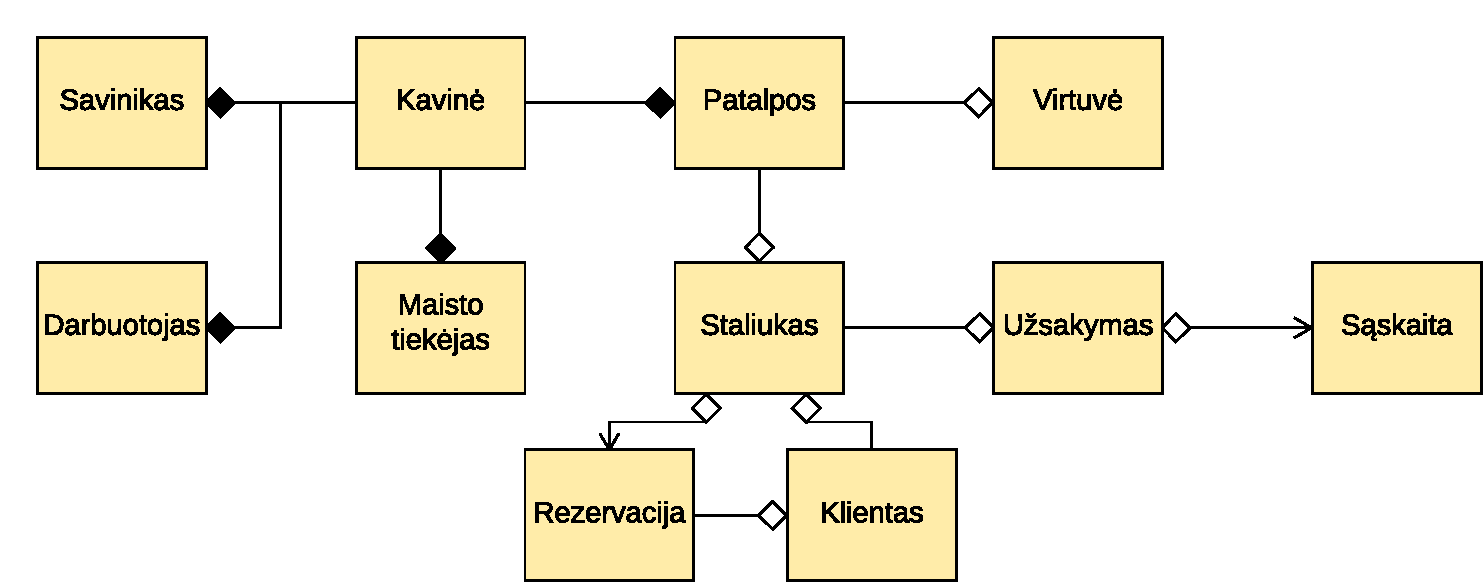
\includegraphics[scale=1]{img/3lab/Diagrama1}
		
		\label{fig:diagrama1}
	\end{figure}
\end{landscape}

Pavaizduota diagrama \ref{fig:diagrama1} pav. pavaizduoja kavinės statinę struktūrą. Kavinė negali egzistuoti be maisto tiekėjų (nebus iš ko ruošti maistą),be darbuotojų (nebus galima efektyviai aptarnauti klientų) ir be kavinės savininko, tad šios esybės sudaro kompoziciją, nes viena negali veikti be kitos.\\
Kavinė gali vykti ir be patalpų, kadangi kavinės staliukai gali stovėti ir 
lauke , todėl šie komponentai sudaro agregaciją.\\
Prie  staliuko  neprivalo  sėdėti  klientas,  nes
staliukas  yra  tik  priemonė  aptarnauti ir jam patogiai jaustis restorane,
klientą.Staliukas taip pat gali nebūti rezervuotas, todėl šios esybės sudaro agregaciją.\\
Patalpose gali būti staliukai ir virtuvė, tačiau tai nėra būtina sąlyga, todėl tai sudaro 
agregaciją.\\
Užsakymas konkretizuoja esybę staliukas.\\
Sąskaita seka po to, kai atliekamas užsakymas.\\

\subsection{Užduočių diagrama}
Klientai  yra  agentai,  kurie  naudodamiesi  kavinės  teikiamomis 
paslaugomis  įgyvendina  užduotis - palydėti  atsisėda  prie  staliuko,  atlieka  užsakymus  ir  juos apmoka. \\
Darbuotojas yra agentas, kuris atlieka tokias užduotis kaip palydėti klientą prie staliuko, 
priimti užsakymą, jį paruošti ir priimti apmokėjimą.\\
Maisto tiekėjas yra agentas, kurio užduotis yra pristatyti reikalingas prekes ir produktus kavinei.\\
Kavinės savininkas valdo kavinės išplanavimą ir staliukų išdėstymą kavinėje. Tik kavinės savininkas gali nuspręsti, kur kavinėje bus išdėstomi staliukai.\\
Agentai ir jų užduotys yra pavaizduoti žemiau esančioje dalykinės srities užduočių diagramoje (žr. \ref{fig:diagrama2} pav).\\


	\begin {figure}[H]
	\centering
		\caption{Dalykinės srities užduočių diagrama}
		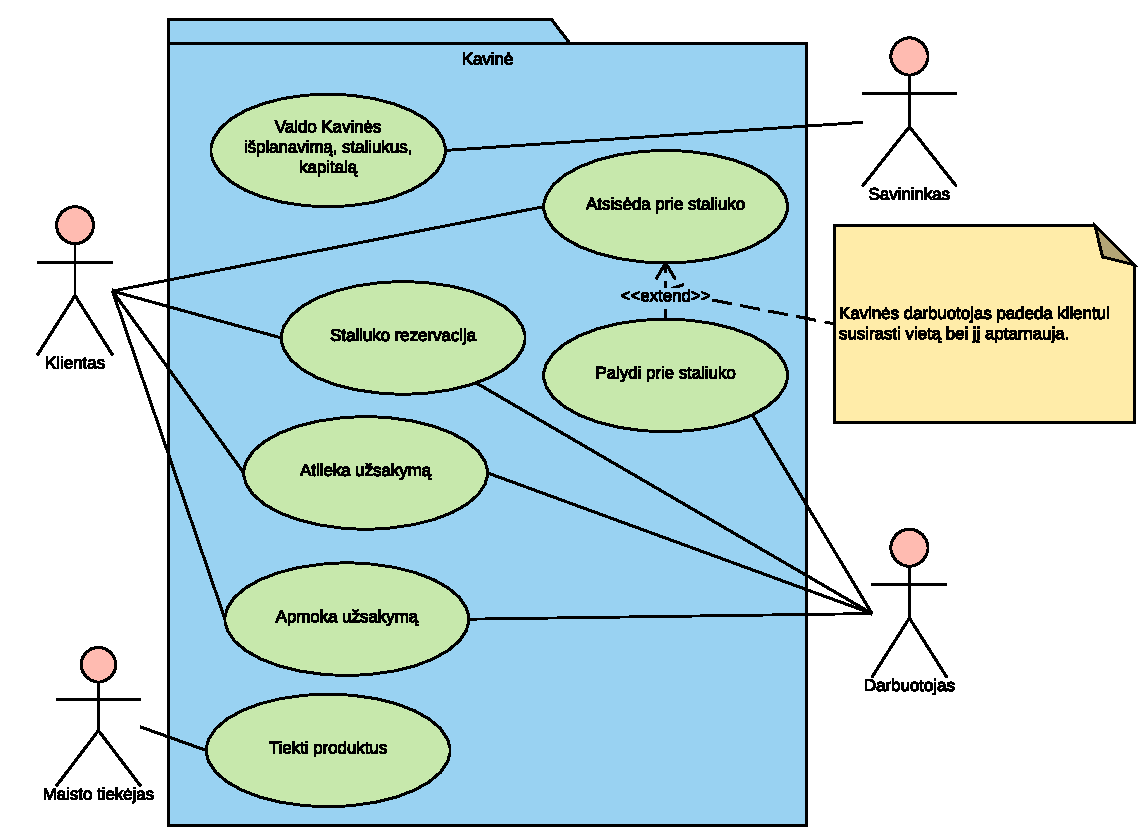
\includegraphics[scale=0.9]{img/3lab/Diagrama2}
		
		\label{fig:diagrama2}
	\end{figure}

\subsection{Užduočių vykdymo scenarijai}
%Insert pauliaus diagram3 here

	\begin {figure}[H]
	\centering
		\caption{Kliento atėjimo į kavinę vykdymo scenarijai}
		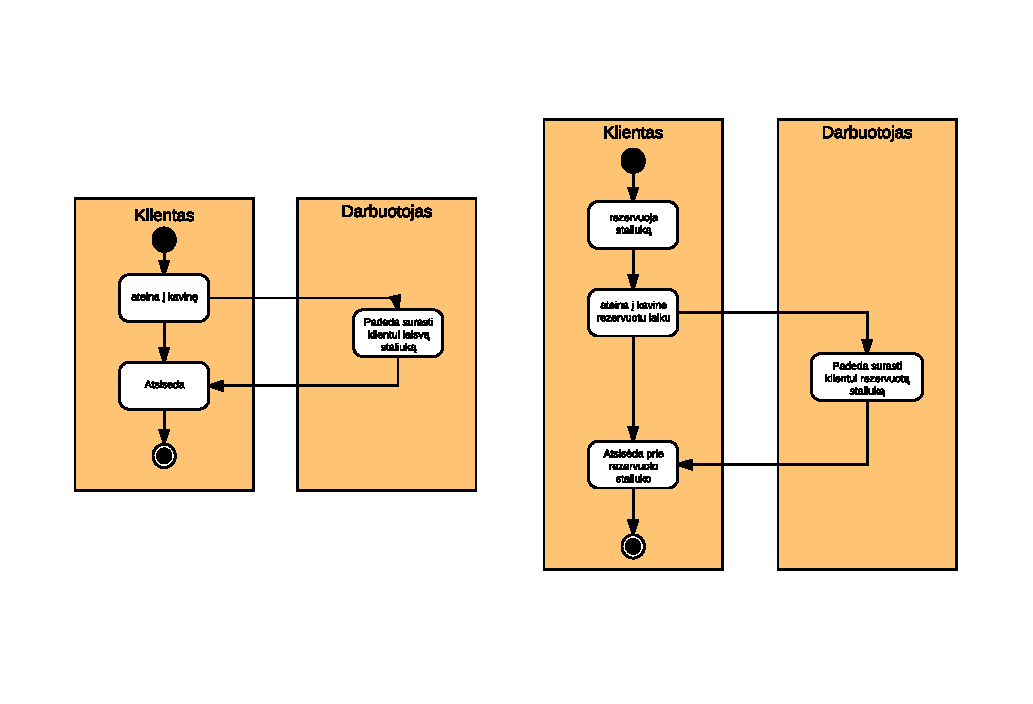
\includegraphics[scale=0.9]{img/3lab/Diagrama3}
		
		\label{fig:diagrama3}
	\end{figure}

Aukščiau pateiktoje užduočių diagramose (\ref{fig:diagrama3}) pavaizduoti kliento be ir su rezervacija užduočių scenarijai.\\ 
Agentas (klientas) ateina į kavinę ir (turėdamas arba neturėdamas rezervacija) gali paprašyti pagalbos darbuotojo,kad padėtų jam rastų staliuką. Klientas gali ir pats susirasti savo staliuką (klientas, neturėdamas rezervacijos, negali atsisėsti į rezervuotą staliuką). \\
Darbuotojas esant poreikiui iš kliento, padeda jam susirasti norimą staliuką: jeigu klientas turi rezervaciją, tai darbuotojas suranda kliento rezervuotą staliuką, jeigu klientas neturi rezervacijos, tai darbuotojas suranda klientui staliuką, kuris nėra rezervuotas tuo metu.\\

%Insert pauliaus diagram4 here

	\begin {figure}[H]
	\centering
		\caption{Kliento atėjimo į kavinę vykdymo scenarijai}
		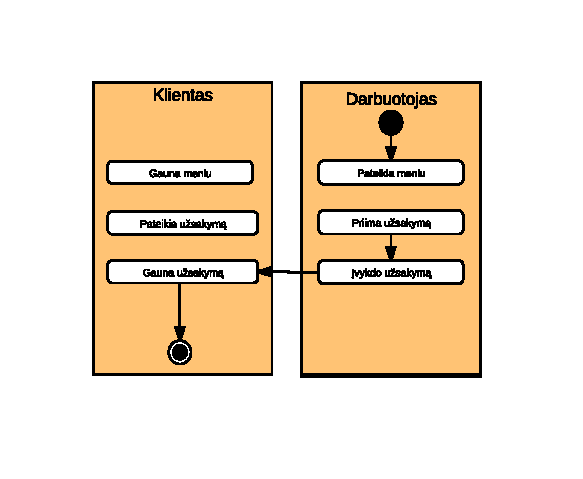
\includegraphics[scale=0.9]{img/3lab/Diagrama4}
		
		\label{fig:diagrama4}
	\end{figure}

Agentas (darbuotojas) pateikia kitam agentui (klientui) meniu. Gavęs meniu, klientas pateikia 
darbuotojui užsakymą ir šis jį priima. Po to, kai priima užsakymą, darbuotojas jį įvykdo ir tuomet klientas gauna įvykdytą užsakymą. \\

%Insert pauliaus diagram5 here

Agentas (klientas) paprašo sąskaitos, tada kitas agentas(darbuotojas) jam ją pateikia. Klientas gauna sąskaitą ir susimoka už jam suteiktas paslaugas. Darbuotojas šį apmokėjimą apdoroja, t.y. jį priima.

\subsection{Dalykinės srities dinaminė struktūra}

%Insert pauliaus diagram6 here
Pradinė  staliuko  būsena  - neužimtas.  Iš  šios  būsenos  staliukas  gali  tapti  užimtas  arba nebenaudojamas. Iš būsenos užimtas staliukas gali pereiti tik į būseną užimtas. 


%Insert pauliaus diagram7 here

Pradinė užsakymo būsena - “pateiktas”, kadangi užsakymas pradeda egzistuoti, kai klientas jį pateikia darbuotojui. Darbuotojui užsirašius ir perdavus užsakymą virtuvei, jis pereina į būseną “priimtas”. Jei užsakymas neįvykdytas, jis nustoja galioti, kitu atveju užsakymas  tampa “paruoštas”. Paruoštas užsakymas yra pristatomas klientui ir keičia būseną į “pristatytas klientui”. Šis turi galimybę arba užsisakyti ką nors papildomai, arba apmokėti sąskaitą. Kai sąskaita apmokama, būsena pasikeičia į „apmokėtas“.\\
\section{Analizės rezultatai}

\section{Verslo proceso tobulinimo strategija}
\noindent \textbf{Vizija}.\\
Visi restorano maisto užsakymo ir tiekimo komponentai(užsakymai vietoje, telefonu, internetu, mobilia programėle, maisto tiekimas vietoje bei į namus) turi atnešti pelno restoranui.\\
\textbf{Misija}.\\
Gerinti maisto tiekimo sąlygas klientams, naudojantis šiuolaikinėmis technologijomis, tobulinti mažiau pelningus komponentus.\\
\textbf{Tikslai/Siekiai}.\\
Didinti restorano staliukų užimtumą, lanksčiai paskirstant klientų srautus:
	\begin{itemize}
	\item Gerinti maisto kokybę ieškaint naujų tiekėjų;
	\item Sumažinti klientų aptarnavimo trukmę;
	\item Pagerinti klientų aptarnavimo kokybę;
	\item Didinti algas restorano darbuotojams;
	\item Didinti klientų užimtumą laukimo metu (plėsti pramogų skaičių, tokių kaip mokami stalo žaidimai ir kt.);
	\end{itemize}
Plėsti užsakymo „iš namų“ sistemą, kuriant internetinę svetainę ar mobilią programėlę, kurios leistų:
	\begin{itemize}
	\item Žemėlapyje parodytų arčiausiai esančius restoranus ir jų laisvų staliukų skaičių;
	\item Matyti restorano staliukų išplanavimą bei kurie staliukai restorane nėra užimti,
	\item Rezervuoti staliuką restorane norimu laiku tam tikroje vietoje;
	\end{itemize}

\section{Sistemos naudojimo scenarijai}

\section{Įgyvendinamumo ir naudos analizė}

\section{Literatūros sąrašas}


\end{document}
